\section{MC Class Reference}
\label{classMC}\index{MC@{MC}}
{\tt \#include $<$MC.h$>$}

Collaboration diagram for MC:\nopagebreak
\begin{figure}[H]
\begin{center}
\leavevmode

\includegraphics[width=400pt]{classMC__coll__graph}
\end{center}
\end{figure}
\subsection*{Public Member Functions}
\begin{CompactItemize}
\item 
void {\bf Init} ()
\item 
void {\bf StartRefresh} ()
\item 
{\bf $\sim$MC} ()
\item 
void {\bf sim\_\-main} ({\bf IrisEvent} $\ast$e)
\end{CompactItemize}
\subsection*{Public Attributes}
\begin{CompactItemize}
\item 
{\bf NI} $\ast$ {\bf ni}
\item 
{\bf RequestHandler} $\ast$ {\bf reqH}
\item 
{\bf RefreshMgr} $\ast$ {\bf refMgr}
\item 
{\bf Bus} $\ast$ {\bf bus}
\item 
{\bf DRAM} $\ast$ {\bf dram}
\item 
{\bf ResponseHandler} $\ast$ {\bf responseH}
\item 
{\bf Statistic} $\ast$ {\bf stats}
\item 
{\bf Component} $\ast$ {\bf parent}
\item 
{\bf UInt} {\bf id}
\end{CompactItemize}


\subsection{Detailed Description}


Definition at line 35 of file MC.h.

\subsection{Constructor \& Destructor Documentation}
\index{MC@{MC}!$\sim$MC@{$\sim$MC}}
\index{$\sim$MC@{$\sim$MC}!MC@{MC}}
\subsubsection[{$\sim$MC}]{\setlength{\rightskip}{0pt plus 5cm}MC::$\sim$MC ()\hspace{0.3cm}{\tt  [inline]}}\label{classMC_c0e7c0a5f6f63dde3189b0349d425322}




Definition at line 59 of file MC.h.

References bus, dram, refMgr, reqH, and responseH.

\subsection{Member Function Documentation}
\index{MC@{MC}!Init@{Init}}
\index{Init@{Init}!MC@{MC}}
\subsubsection[{Init}]{\setlength{\rightskip}{0pt plus 5cm}void MC::Init ()}\label{classMC_05109b1e9678c5d598027d7c47d7b2a4}




Definition at line 20 of file MC.cc.

References bus, ResponseHandler::child, RequestHandler::child, Bus::child1, Bus::child2, dram, Statistic::InitStats(), Statistic::mc, RefreshMgr::mc, ResponseHandler::mc, DRAM::mc, Bus::mc, RequestHandler::mc, ni, ResponseHandler::parent, DRAM::parent, Bus::parent, RequestHandler::parent, refMgr, reqH, RefreshMgr::reqPtr, ResponseHandler::reqPtr, responseH, RequestHandler::resPtr, DRAM::SetLinks(), Bus::SetLinks(), RequestHandler::SetLinks(), StartRefresh(), and stats.

Referenced by main().

Here is the caller graph for this function:\nopagebreak
\begin{figure}[H]
\begin{center}
\leavevmode
\includegraphics[width=85pt]{classMC_05109b1e9678c5d598027d7c47d7b2a4_icgraph}
\end{center}
\end{figure}
\index{MC@{MC}!sim\_\-main@{sim\_\-main}}
\index{sim\_\-main@{sim\_\-main}!MC@{MC}}
\subsubsection[{sim\_\-main}]{\setlength{\rightskip}{0pt plus 5cm}void MC::sim\_\-main ({\bf IrisEvent} $\ast$ {\em e})}\label{classMC_bf467a900cc11b932afd0e7432dd504c}




Definition at line 112 of file manifold\_\-simmc.cc.

References CONTINUE, IrisEvent::dst, IrisEvent::event\_\-data, GetNextRequest(), Simulator::Now(), RequestHandler::oneBufferFull, RequestHandler::process\_\-event(), reqH, Simulator::Schedule(), IrisEvent::src, START, and IrisEvent::type.

Referenced by main().

Here is the caller graph for this function:\nopagebreak
\begin{figure}[H]
\begin{center}
\leavevmode
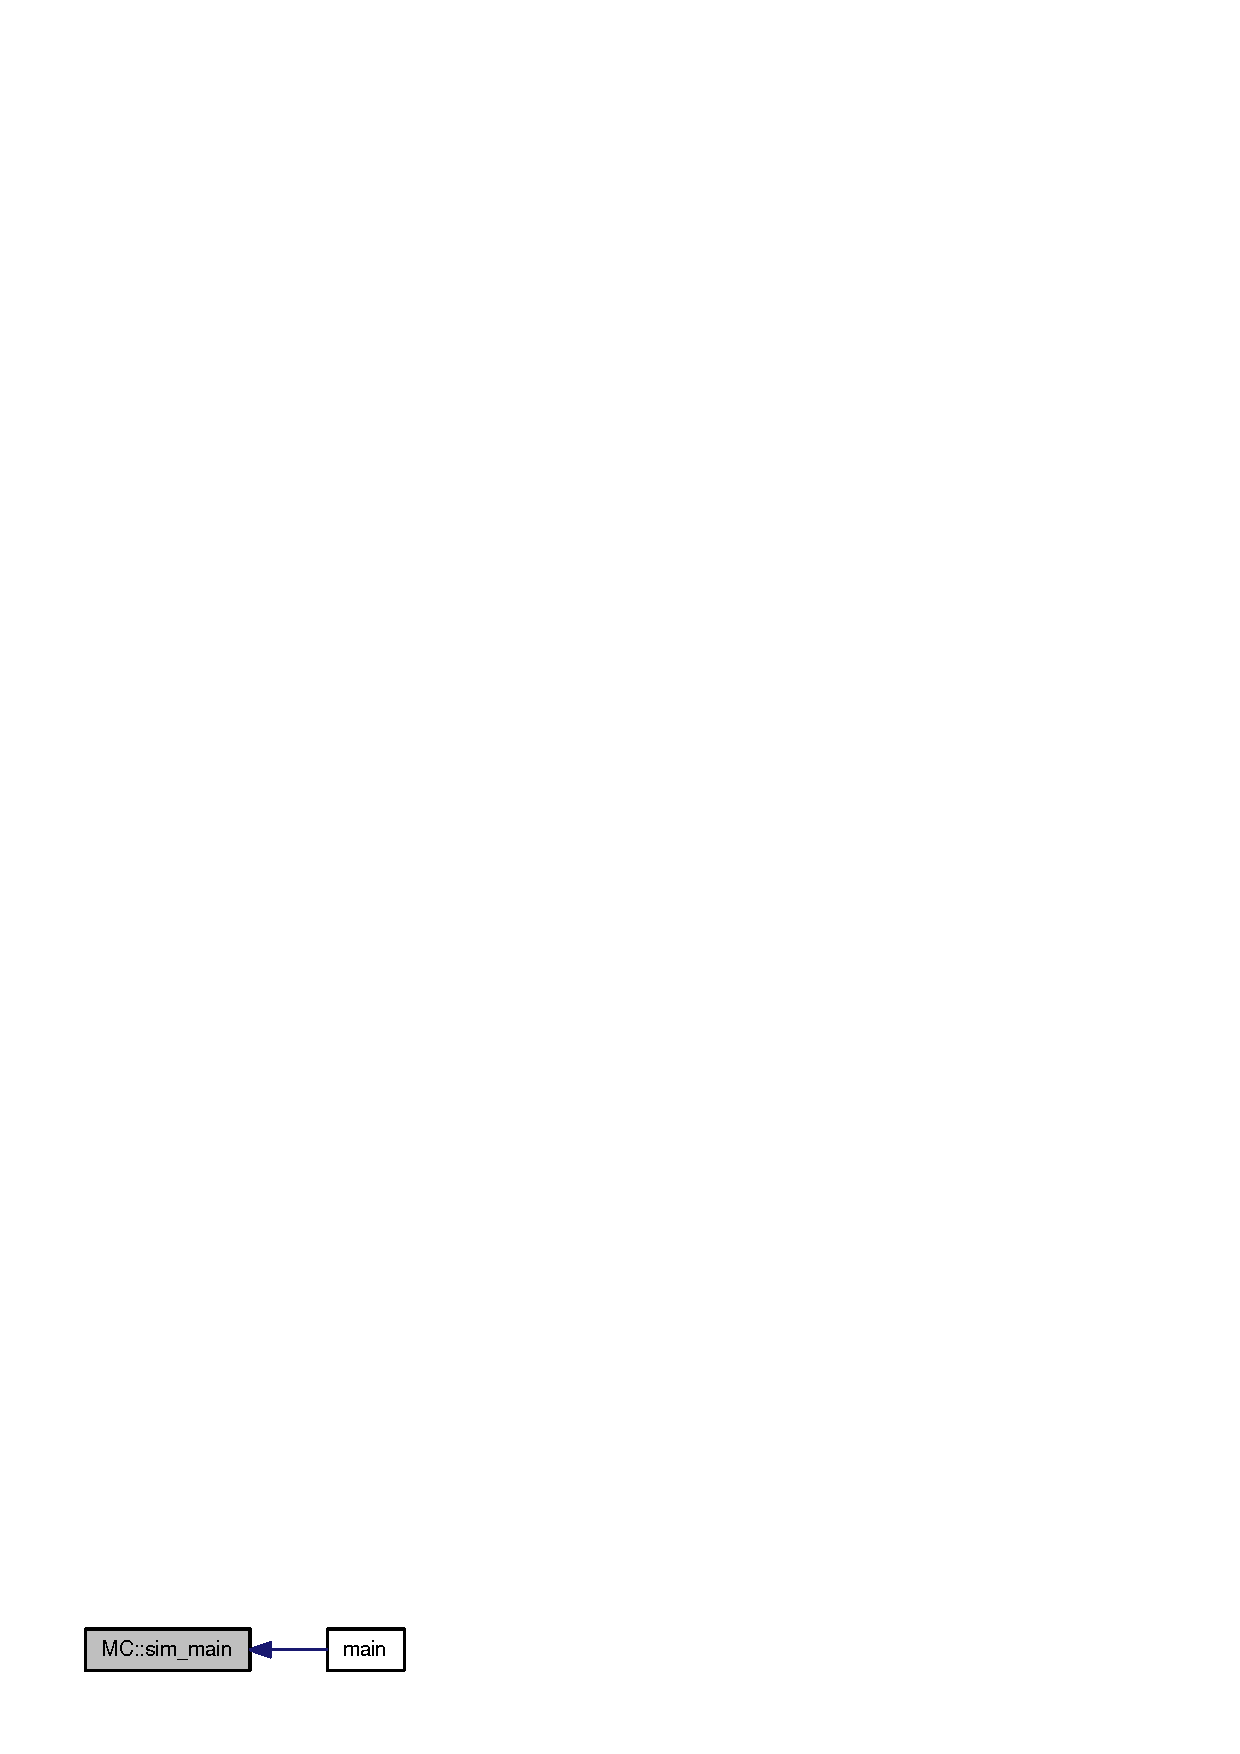
\includegraphics[width=99pt]{classMC_bf467a900cc11b932afd0e7432dd504c_icgraph}
\end{center}
\end{figure}
\index{MC@{MC}!StartRefresh@{StartRefresh}}
\index{StartRefresh@{StartRefresh}!MC@{MC}}
\subsubsection[{StartRefresh}]{\setlength{\rightskip}{0pt plus 5cm}void MC::StartRefresh ()}\label{classMC_1f4c68b63112b1bd4fa8bcdf47a8e57c}




Definition at line 48 of file MC.cc.

References RefreshMgr::nextRefresh, Simulator::Now(), RefreshMgr::process\_\-event(), refMgr, REFRESH\_\-INC, and Simulator::Schedule().

Referenced by Init().

Here is the caller graph for this function:\nopagebreak
\begin{figure}[H]
\begin{center}
\leavevmode
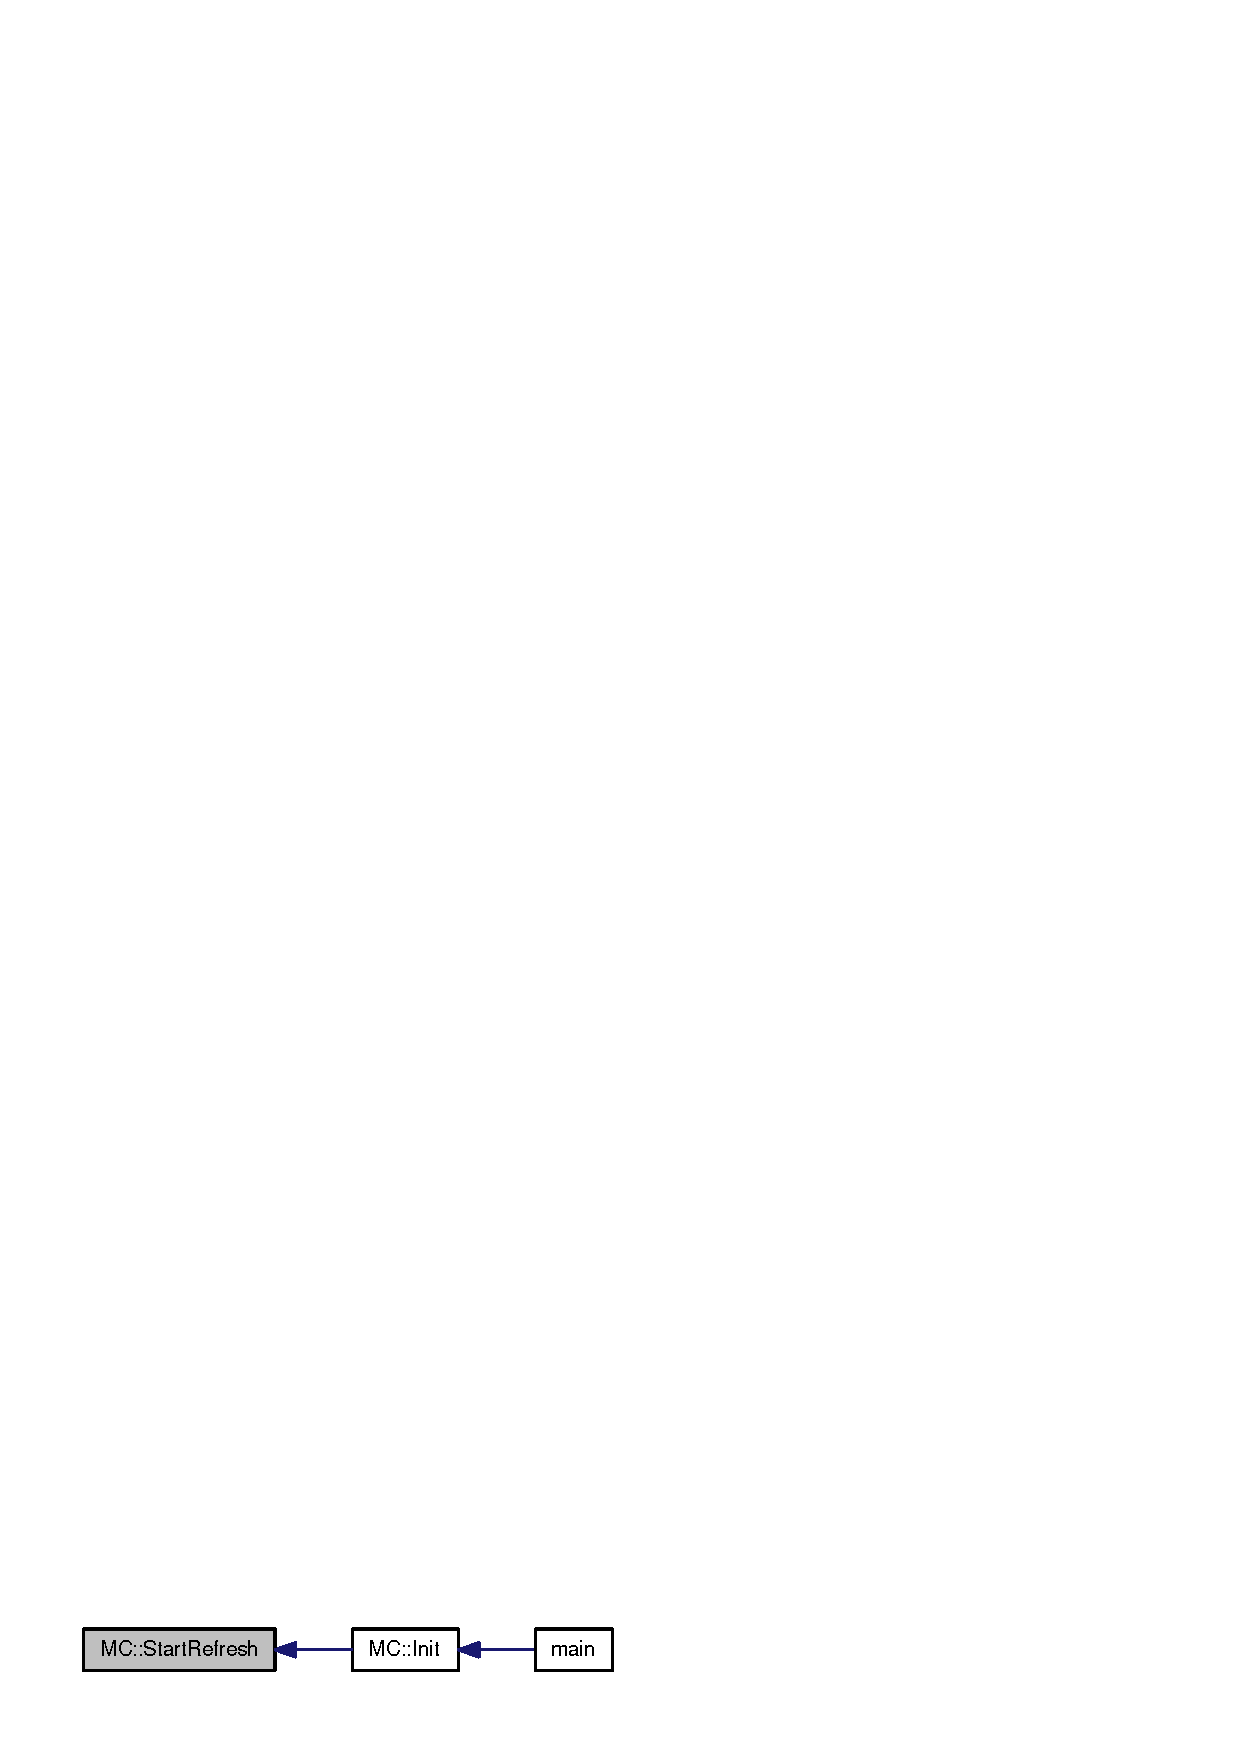
\includegraphics[width=149pt]{classMC_1f4c68b63112b1bd4fa8bcdf47a8e57c_icgraph}
\end{center}
\end{figure}


\subsection{Member Data Documentation}
\index{MC@{MC}!bus@{bus}}
\index{bus@{bus}!MC@{MC}}
\subsubsection[{bus}]{\setlength{\rightskip}{0pt plus 5cm}{\bf Bus}$\ast$ {\bf MC::bus}}\label{classMC_5e52255c7c0f51558148857c35c5b233}




Definition at line 41 of file MC.h.

Referenced by Init(), and $\sim$MC().\index{MC@{MC}!dram@{dram}}
\index{dram@{dram}!MC@{MC}}
\subsubsection[{dram}]{\setlength{\rightskip}{0pt plus 5cm}{\bf DRAM}$\ast$ {\bf MC::dram}}\label{classMC_f809d7e712e3b14f455f9945a4f70cd8}




Definition at line 42 of file MC.h.

Referenced by Init(), and $\sim$MC().\index{MC@{MC}!id@{id}}
\index{id@{id}!MC@{MC}}
\subsubsection[{id}]{\setlength{\rightskip}{0pt plus 5cm}{\bf UInt} {\bf MC::id}}\label{classMC_44f183ff320c8100d4d7bbe9cd2f2086}




Definition at line 49 of file MC.h.\index{MC@{MC}!ni@{ni}}
\index{ni@{ni}!MC@{MC}}
\subsubsection[{ni}]{\setlength{\rightskip}{0pt plus 5cm}{\bf NI}$\ast$ {\bf MC::ni}}\label{classMC_b91265d7b3e979122d20de7abfc6d854}




Definition at line 38 of file MC.h.

Referenced by Init(), and main().\index{MC@{MC}!parent@{parent}}
\index{parent@{parent}!MC@{MC}}
\subsubsection[{parent}]{\setlength{\rightskip}{0pt plus 5cm}{\bf Component}$\ast$ {\bf MC::parent}}\label{classMC_bf2f57e15f676b20c0b0e9eb6b1880fe}




Definition at line 45 of file MC.h.\index{MC@{MC}!refMgr@{refMgr}}
\index{refMgr@{refMgr}!MC@{MC}}
\subsubsection[{refMgr}]{\setlength{\rightskip}{0pt plus 5cm}{\bf RefreshMgr}$\ast$ {\bf MC::refMgr}}\label{classMC_e273df8dc1334a025db110d21ba90bca}




Definition at line 40 of file MC.h.

Referenced by Init(), StartRefresh(), and $\sim$MC().\index{MC@{MC}!reqH@{reqH}}
\index{reqH@{reqH}!MC@{MC}}
\subsubsection[{reqH}]{\setlength{\rightskip}{0pt plus 5cm}{\bf RequestHandler}$\ast$ {\bf MC::reqH}}\label{classMC_95b5a37c33fa8a000ec0969abdde0118}




Definition at line 39 of file MC.h.

Referenced by Init(), main(), sim\_\-main(), and $\sim$MC().\index{MC@{MC}!responseH@{responseH}}
\index{responseH@{responseH}!MC@{MC}}
\subsubsection[{responseH}]{\setlength{\rightskip}{0pt plus 5cm}{\bf ResponseHandler}$\ast$ {\bf MC::responseH}}\label{classMC_ce4c1e78e98a11a6f1f64284e89832e9}




Definition at line 43 of file MC.h.

Referenced by Init(), and $\sim$MC().\index{MC@{MC}!stats@{stats}}
\index{stats@{stats}!MC@{MC}}
\subsubsection[{stats}]{\setlength{\rightskip}{0pt plus 5cm}{\bf Statistic}$\ast$ {\bf MC::stats}}\label{classMC_60c08c4803f1e4117fd6cb8a5b1d5052}




Definition at line 44 of file MC.h.

Referenced by Init(), and main().

The documentation for this class was generated from the following files:\begin{CompactItemize}
\item 
{\bf MC.h}\item 
{\bf manifold\_\-simmc.cc}\item 
{\bf MC.cc}\end{CompactItemize}
